\section{System-level Design}

\subsection{Testbench Architecture}
The design of the verification system is the major engineering challenge of this
project.
While there have been many similar performance analyses done on hybrid SoCs
before, each of them used their own, usually ad hoc, testbench
design~\cite{Shi1}~\cite{Li1}.
As such, most testbench are not designed to be scalable or portable, serving
only what they are built for.
In this project, I shall use a generic structure inspired by that of an agent
in Universal Verification Methodology (UVM).

Before UVM, integrated circuit designs were verified with methodologies
developed independently by stimulator vendors such as Cadence, Mentor Graphics,
and Synopsys.
In an effort to unify for greater efficiency, the standards organisation of the
Electronic Design Automation (EDA) industry, Accellera, established UVM with
support from multiple vendors.
It provided a common structure for verification, with class libraries that made
building and running a testbench a significantly smoother experience.
The agent is a container in UVM that emulates and verifies
DUTs~\cite{Accellera1}.
While this project is in no position to achieve what UVM has done, I do hope
that this testbench would have an easily modifiable structure that will make
the process of testing similar future designs slightly simpler.

\begin{figure}[H]
  \centering
  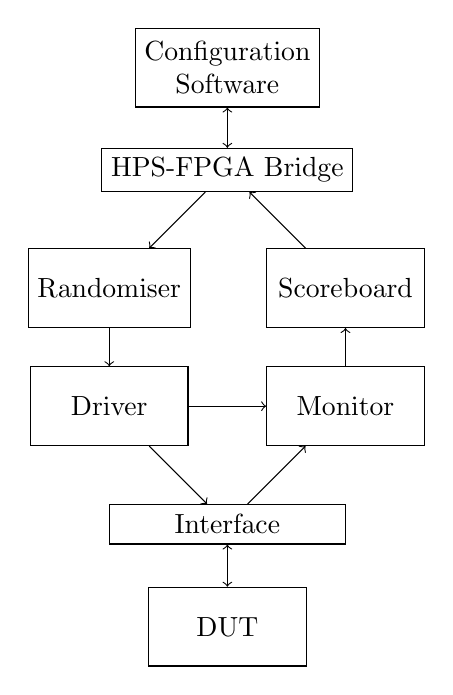
\begin{tikzpicture}
    \tikzset{block/.style= {draw,
                            rectangle,
                            align=center,
                            minimum width=2cm,
                            minimum height=1cm},
             inter/.style= {draw,
                            rectangle,
                            minimum width=3cm,
                            minimum height=0.5cm},
            }
    \path
    (0,3.5)    node[block](r) {Randomiser}
    (0,2)      node[block](d) {Driver}
    (1.5,0.5)  node[inter](i) {Interface}
    (1.5,-0.8) node[block](t) {DUT}
    (3,3.5)    node[block](s) {Scoreboard}
    (3,2)      node[block](m) {Monitor}
    (1.5,5)    node[inter](b) {HPS-FPGA Bridge}
    (1.5,6.3)  node[block](w) {Configuration\\Software}
    ;
    \draw[->]  (r) -- (d);
    \draw[->]  (d) -- (i);
    \draw[<->] (i) -- (t);
    \draw[->]  (i) -- (m);
    \draw[->]  (m) -- (s);
    \draw[->]  (b) -- (r);
    \draw[->]  (s) -- (b);
    \draw[<->] (b) -- (w);
    \draw[->]  (d) -- (m);
\end{tikzpicture}
  \caption{Block diagram of the proposed testbench}
  \label{Block}
\end{figure}

Configuration is first done from software running on the HPS, which sends
the test specifications to the randomiser.
The randomiser will provide a stream of random data that will be converted
to meaningful test inputs by the driver.
The test output will be watched by the monitor, reporting any interesting
event to the scoreboard, which keeps track of them.
The scoreboard feeds the information back to the software on demand.
The interface is used to decouple the control logic from the DUT, allowing
the frequency of the DUT to be finely controlled.

\subsection{User Interface}
